\chapter{A Visualization Framework for Dark Matter Simulation Data}

\section{Introduction}

Dark matter, the unidentified substance that comprises the vast majority of matter in the universe, generates a wealth of unanswered questions for scientists. Dark matter is invisible, interacting only via gravitational force; for now, it must be modeled with large-scale simulations. These simulations play a major role in furthering our understanding of the universe's history and provide insight into various astrophysical phenomena. As a result, vast effort goes toward developing large-scale N-body simulation frameworks to study universe formation. One such framework, HACC (Hardware/Hybrid Accelerated Cosmology Code)~\cite{Habib:2014}, has been used to push the scale of simulations ever-larger. Various cosmological simulations such as ``Q Continuum''~\cite{Heitmann:2014} (which utilizes HACC), ``DarkSky''~\cite{Skillman:2014}, and ``Millenium''~\cite{Angulo:2013} have contributed vast amounts of data for interpretation by the scientific community. Their eventual goal is to map raw data onto observable features of the universe with measurable physical properties, which can then be compared with observations and used to develop theories or further refine simulation code. Simulations are crucial in preparing data analysis techniques for upcoming sky surveys such as LSST (2022)~\cite{LSST}, which will produce up to 15 TB of data every night, totaling 100 PB of images over its planned ten-year duration.

The size of a simulation, dictated by its number of particles and mass resolution (the smallest mass unit represented), has strong implications for its ability to provide useful information. For example, in order to trace the behavior of bright galaxies, a simulation must contain at least one hundred dark matter particles per galaxy. Furthermore, in order to study structure formation via halo mergers, the simulation must have a mass resolution fine enough to capture low-mass halos that are just beginning to form. These two factors drive the massive scale of cosmological simulation data, leading to simulation sizes of hundreds of billions to trillions of particles at present~\cite{skysurvey}. Such large scales make analysis and visualization difficult in an interactive setting. This work presents a novel integrated visualization system for the interactive analysis of raw and derived cosmology simulation data. Through use of a parallelized remote renderer, as well as a carefully designed merger tree visualization and selection tool, we provide the means to simultaneously study multiple aspects of vast cosmological simulation datasets in real time.

In this study, we focus on enabling scientists to analyze extracted data from cosmological simulations since this area is highly relevant to upcoming observational data. We present our visualization system, demonstrate its effectiveness through a set of case studies using large-scale simulation data, and make the following contributions:

\vspace{-0.9\topsep}
\begin{itemize} \itemsep1pt \parskip1pt \parsep1pt
  \item We develop a coherent and interactive visualization system in close collaboration with domain scientists aimed at exploring heterogeneous cosmology data.
  \item We offer the ability to gain new, visually guided insights into the behavior of large scale simulations, which in turn illuminate data results from observational surveys.
  \item We provide the means for expert users to assess the quality of halo-finding and merger tree extraction algorithms.
\end{itemize}
\vspace{-0.9\topsep}

\section{Background and Related Work}
Cosmological simulations produce a multitude of heterogeneous data types that must be analyzed simultaneously in order to thoroughly investigate phenomena of interest. The primary output from these simulations is a time-varying particle-based representation of the dark matter distribution throughout the universe.

\subsection{Halos and Halo Finding}
Over time, mutual gravitation among dark matter particles causes them to collapse into larger structures. The individual groups of gravitationally bound particles that form in this process are called halos. Applying a halo-finding algorithm to the raw data yields a catalog of dark matter halos at each timestep (Figure \ref{fig:halo_explanation}).

Halo finding, an example of feature extraction, is essential for analyzing the output of cosmological simulations. One popular halo finding algorithm, Rockstar~\cite{Behroozi:2013}, uses a hierarchical technique to locate halos. Large halos are quickly identified and then adaptively refined into subgroups with progressively smaller linking lengths. This outputs a set of halos once a desired level of detail is reached. Widanagamaachchi et al.~\cite{Widanagamaachchi:2014} developed a highly parallel halo extraction algorithm which is also flexible enough to extract features without choosing a specific linking length. Though most halo-finding techniques utilize mass density, Popov et al.~\cite{Popov:2011} utilize a velocity-based technique to extract a wider range of features. A survey by Knebe at al.~\cite{Knebe:2011} explores other techniques.

	\begin{figure}[t]
		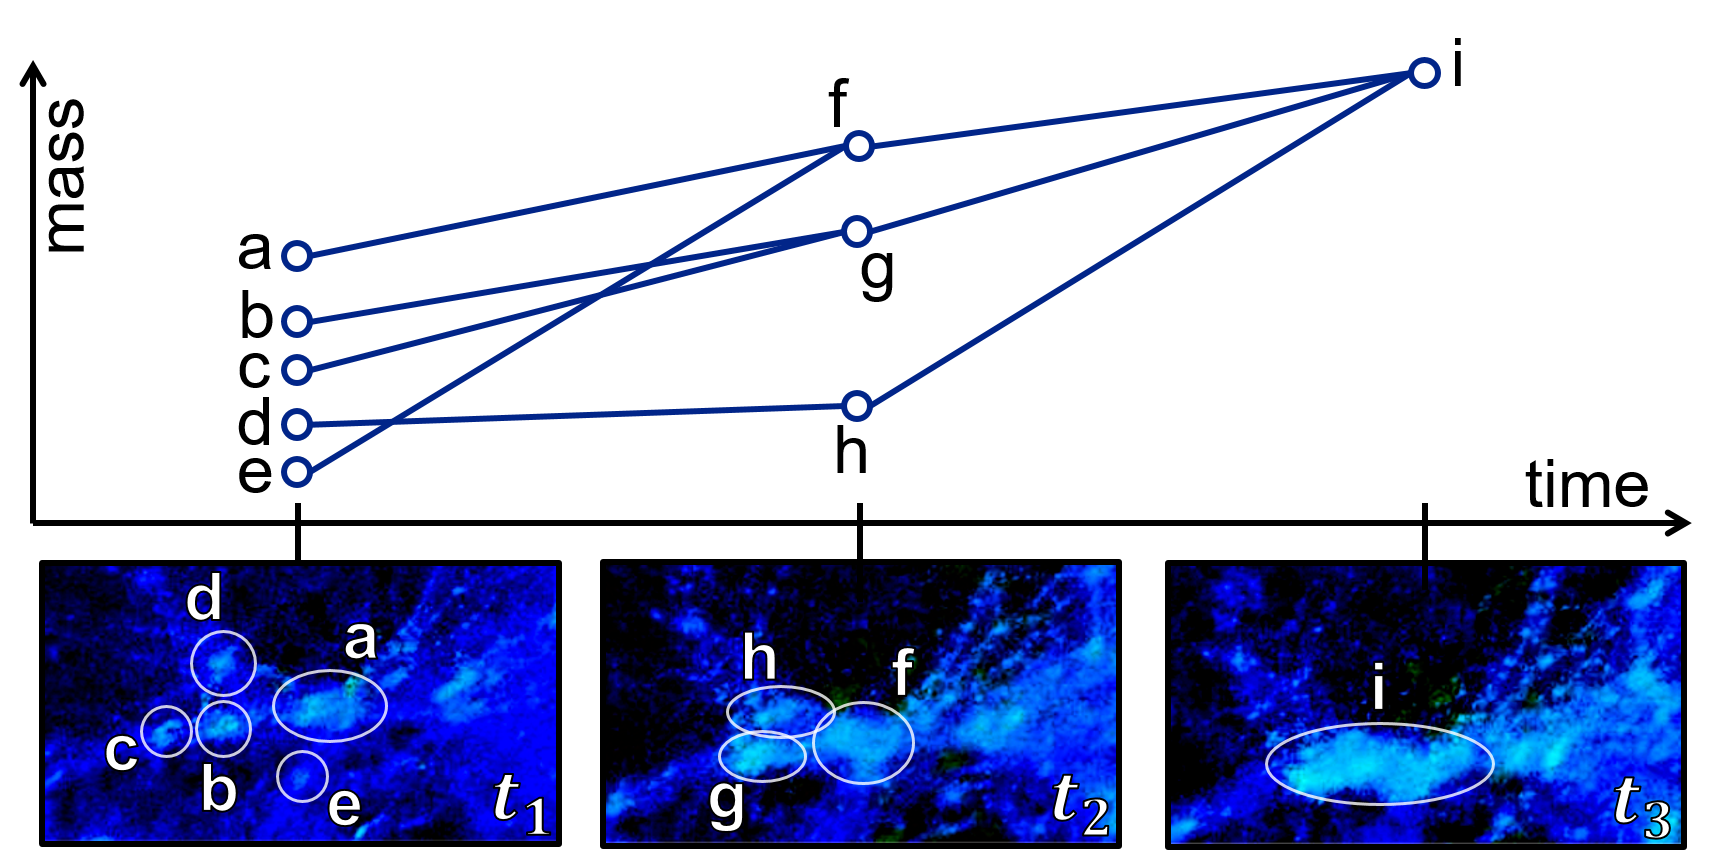
\includegraphics[width=\textwidth]{images/darkmatter/halo_explanation_4}
		\caption{The process of extracting merger trees from simulation output. Below, we see the same spatial domain at three timesteps. Over time, the particles coalesce into larger structures. A friends-of-friends algorithm identifies these groups of particles, called halos, at each timestep. The merger tree above shows halos (nodes) linked by edges which indicate the halos they merge into in subsequent timesteps.}
		\label{fig:halo_explanation}
	\end{figure}

\subsection{Merger Trees}
Once dark matter halos are extracted, they are associated across time steps to create halo merger trees~\cite{skysurvey}. These trees capture the way that halos form over time (Figure \ref{fig:halo_explanation}). The dark matter particles within encode information about the formation of structures, specifically galaxies, in the universe, a phenomenon that is currently poorly understood. Effectively visualizing the interplay between particle data, halo data, and their hierarchical evolution (as represented by a merger tree) can allow researchers to intuitively explore connections and draw conclusions.

In addition to a static visualization of halos and extracted features, researchers need to study their time-varying evolution. Shan et al.~\cite{Shan:2014} utilize a tree-like visualization view, which describes mergers linked with a 3D visualization of particle tracers to study halo evolution. In their scheme, users select halos in the 3D view, which results in the corresponding merger trees being shown in a graph layout. Our system allows selection of specific halos through the merger trees themselves, as well as using physical variables (such as velocity or mass) for laying out and organizing the merger trees. Takle et al.~\cite{Tackle:2012} developed a multilevel method of tracking the evolution and mergers of groups of dark matter tracer particles (called satellite halos) and groups of satellite halos (called host halos), visualizing these structures in isolation. Such a multilevel approach is useful since structures that interest cosmologists often occur across multiple scales. We expand upon their capability by including interactive selection as well as showing the broader context of each halo within the simulation domain.

\subsection{Visualization Techniques}
Once scientists extract features from a simulation, they can use visualization and analysis tools to explore underlying patterns in the data. One difficulty is the extensive amount of multivariate information necessary to fully represent a halo and its properties. Takle et al.~\cite{Tackle:2013} use a glyph-based representation to simultaneously visualize multiple properties of groups of halos. Another key interest lies in representing the physical shape and structure of these point-based representations. Miller et al.~\cite{Miller:2006} address this by using a unique set of 3D projections, as well as geometric glyphs showing potential correlation between galactic clusters. A visualization of the uncertainty in the simulation data is explored in a work by Haroz et al.~\cite{Haroz:2008}. Ahrens et al.~\cite{Ahrens:2006} use comparative visualization to determine subtle differences between different simulation codes using the same initial conditions. In addition, K\"{a}hler and Abel~\cite{Kaehler:2012v2} explore the use of stereoscopic techniques to enhance the perceptual ability of cosmology researchers.

There has also been an effort to generate high-quality renderings of the simulation particle data and extracted halos. K\"{a}hler et al.~\cite{Kaehler:2012} utilize a cell-projection~\cite{max1990area,Rottger2000} technique on a tetrahedral mesh derived from the initial condition of the simulation particles to visualize the dark matter density distributions; we include this method as a supplemental tool in our visualization system. Scalability becomes an issue when generating high quality images in a real-time interactive setting. Fraedrich et al.~\cite{Fraedrich:2009} use an octree based level-of-detail approach in conjunction with GPU data compression to address this problem.

In addition, there have been numerous recent advances in parallel particle rendering in general. For example, Rizzi et al.~\cite{Rizzi:2015} develop a large-scale direct point rendering framework, which uses hierarchical representations and z-ordering for improved load balancing. On the other hand, Stone et al.~\cite{Stone:2013} utilize a ray-tracing method on extracted density maps to visualize complex molecular shapes in petascale applications. In addition, Akinci et al.~\cite{Akinci:2012} use a parallel approach to surface reconstruction of large particle-based fluids based on Marching Cubes to accelerate rendering. Rendering in a distributed setting also requires careful attention to compositing techniques. One notable example, which we use here, is the 2-3 swap method developed by Yu et al.~\cite{23swap}; this efficiently and scalably performs compositing across large numbers of nodes.


\section{System Design}
 Our system design is motivated by the need to simultaneously observe multiple data types, as determined through close collaboration with domain scientists. These include particle data from the simulation, extracted halos, and constructed merger trees. An understanding of the interplay among data types is essential for scientific analysis. Moreover, visualizing the simulation's physical behavior at one timestep is more useful when associated with quantitative and chronological information. Data from the raw particles and the extracted halos inform one another; we enhance these views with both qualitative and quantitative information. Because of the scale of the data and the multitude of features, we aim to provide improved capability to focus analysis on specific features of interest. 

\subsection{System Components}
Figure~\ref{fig:system} shows our visualization system workflow. Since the raw particle data is too large to manage on a single machine, we utilize a remote parallel renderer to visualize the particles. The halo information and merger trees, however, are small enough in scale that they can be transferred to a desktop PC and visualized locally. The interactive visualization system communicates between the local file systems and the remote renderer for seamless exploration of each of the data types. The visualization tool utilizes three main views that can be used to explore the data: a particle explorer for a direct 3D rendering of particle data, a view for the exploration of merger trees, and a quantitative display for plots of halo and particle variables.

	\begin{figure}[t]
		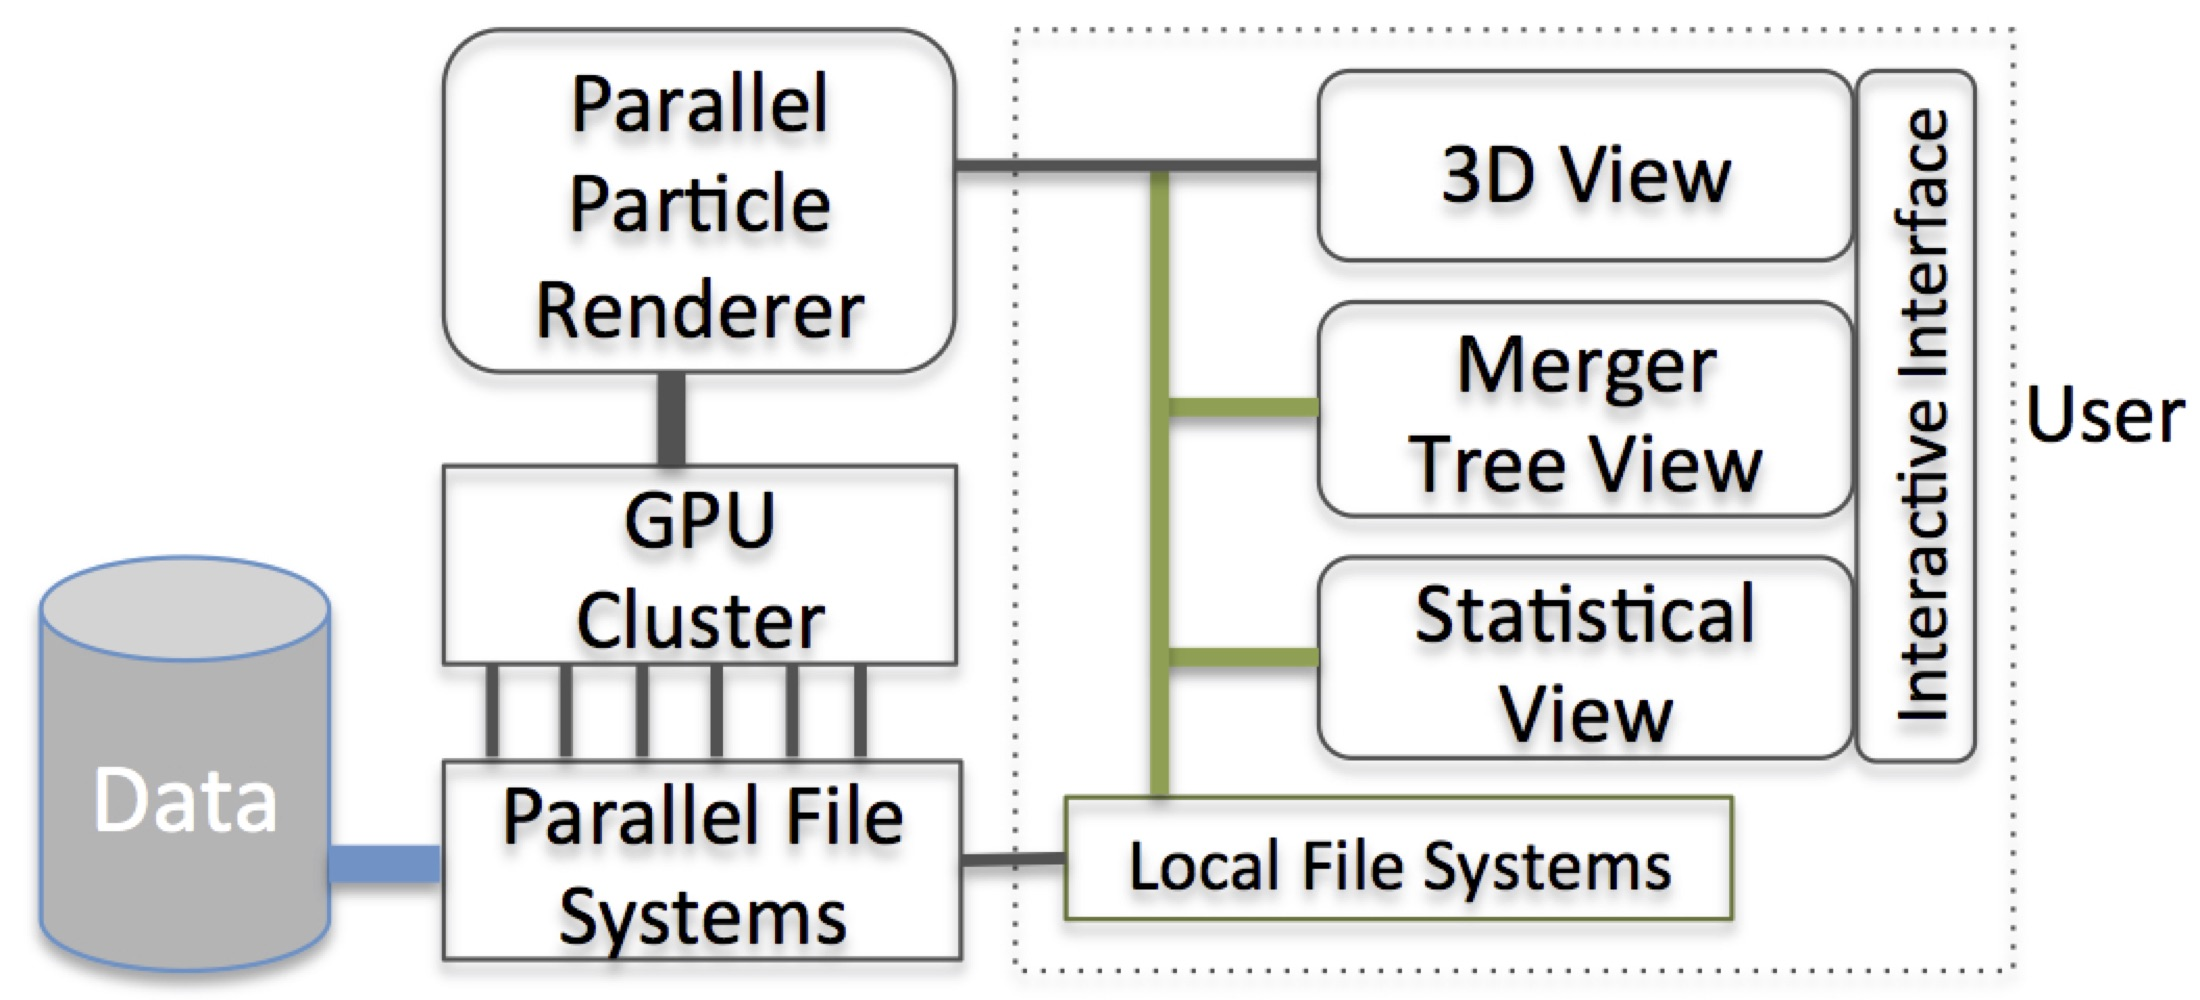
\includegraphics[width=8.5cm]{images/darkmatter/CosmoVis.jpg}
		\centering
		\caption{An overview of the system workflow. The large scale particle data resides in a distributed system and is visualized using a paralleled remote renderer. The smaller scale halo merger tree data resides locally and is rendered using a desktop computer.}
		\label{fig:system}
	\end{figure}

\subsubsection{User Interface}
The user interface (Figure~\ref{fig:ui}) integrates the three visualization tools: the quantitative and 3D particle rendering views are placed in the top right and top left respectively, with the merger tree visualization placed below. The user in this example investigates a subset of the merger trees in velocity space, choosing to view corresponding mass information in the quantitative view. Below the merger tree is a slider for selecting a particular timestep. The tabs beside the quantitative view reveal additional interface elements, such as a transfer function editor for coloring the 3D particles. Each of the views can be resized relative to the others in order to provide additional visual detail when working in that particular view.

	\begin{figure}[t]
		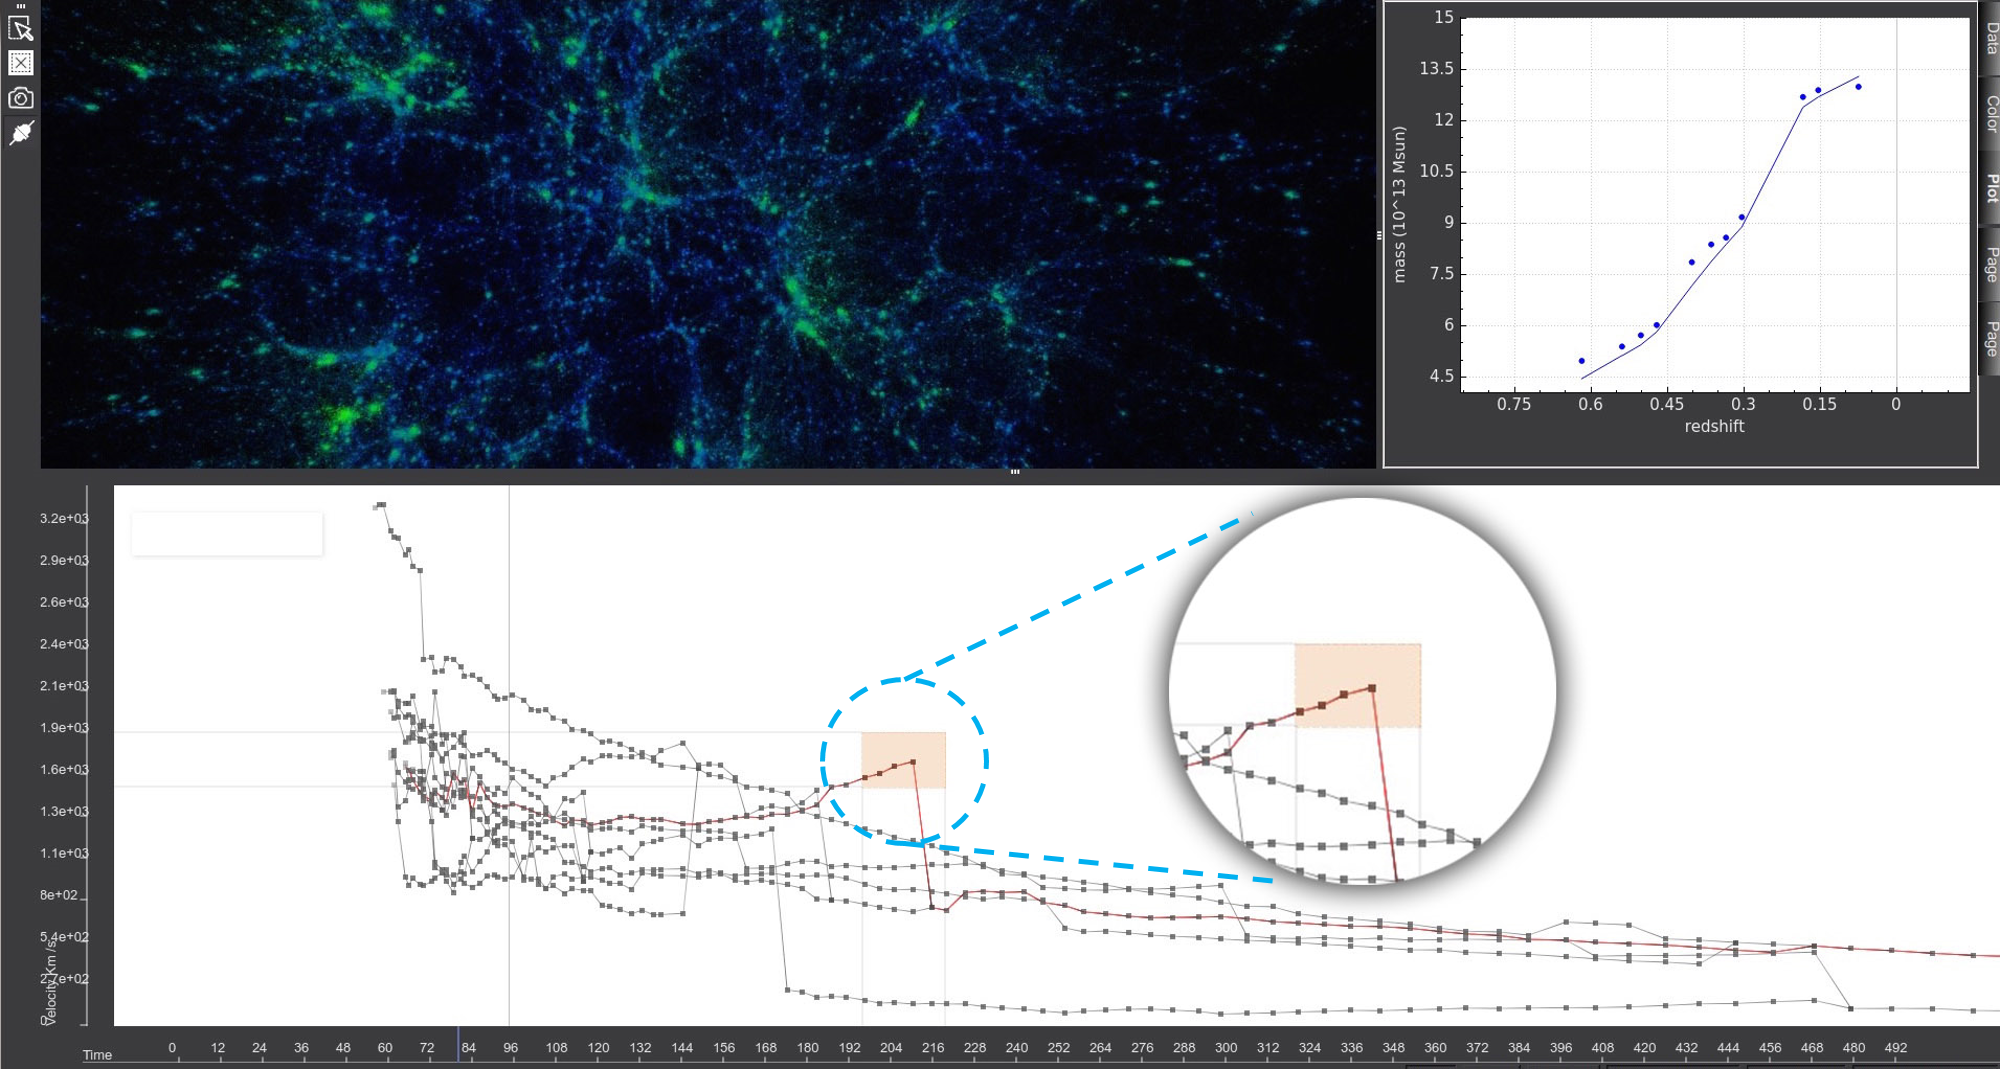
\includegraphics[width=\textwidth]{images/darkmatter/ui_new_zoomin.png}
		\caption{A snapshot of the user interface. The quantitative view and 3D particle rendering are placed on the top right and top left respectively. The merger tree visualization is placed below. Here, the user explores a subset of merger trees. For clarity in this figure, we provide a zoomed-in view of the selection box that the user has drawn.}
		\label{fig:ui}
	\end{figure}

\subsubsection{Merger Tree Visualization}
We provide an interactive visualization and selection tool for the halo merger trees, which are hierarchical representations of the dark matter halo formation histories. Each halo present in the final timestep of the simulation has an associated merger tree describing its past. On average, there is approximately one halo for every thousand particles in the final timestep of the simulation. Given this data size, viewing all the trees simultaneously would not allow for detailed visual analysis of the mergers due to overplotting and clutter. We employ several methods for reducing the number of trees needed for visualization. The user can focus on a single merger tree, progressing through the data one tree at a time. We also provide capability to iteratively select smaller subsets of trees using selection boxes and zooming. Another approach uses lists of interesting halo events that domain scientists identify in postprocessing in order to select a tree or trees of interest. Scientists are particularly interested in merger trees that do not behave as expected; these trees might be reflective of bugs in the halo finder code. For example, a massive halo that suddenly appears in one timestep is not physically feasible, since it must coalesce over time from a mass close to the simulation's minimum mass resolution. We offer the option to select and isolate merger trees based on these anomalous events. Because there are far fewer halos than particles, we can store and visualize the merger tree data at an interactive rate using a local desktop computer.

	\begin{figure}[t]
		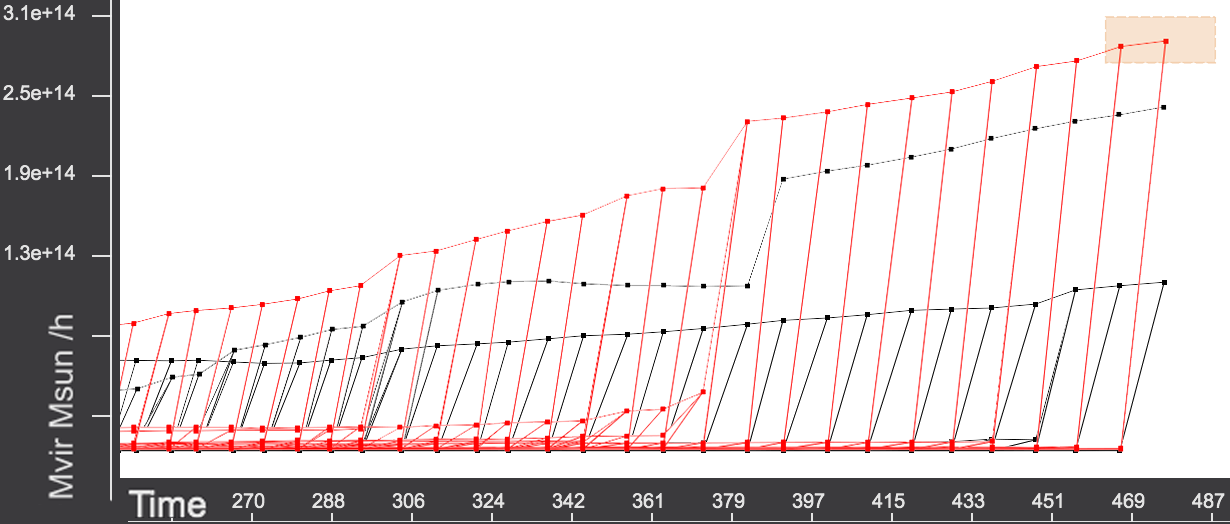
\includegraphics[width=\textwidth]{images/darkmatter/mt_overview.png}
		\caption{Several merger trees (black) with time on the x axis and mass on the y axis. The user chooses a node with the selection box, which highlights all progenitors and descendants leading to and from that node (red). Large vertical jumps represent nodes at which a halo was subsumed into a much larger halo due to gravitational force.}
		\label{fig:mergetreehundred}
	\end{figure}

The merger tree visualization draws the tree structures and allows for interactive exploration (Figure~\ref{fig:mergetreehundred}). While the horizontal axis represents time by default, since temporal evolution is of primary importance, both axes can be mapped to any halo-specific property of interest (e.g., mass or velocity). In addition, our system offers zooming and selection capabilities; the zoom reduces the visible range of timesteps or of the mapped property, while the selection feature allows for highlighting of particular trees or descendant node families. The selection is highlighted and corresponding particle IDs are communicated to the remote particle renderer so that the particles belonging to the selected halos/nodes can be highlighted in 3D space. Lastly, mousing over portions of the merger tree will display additional relevant information for that particular node.

\subsubsection{3D Rendering}
This view offers context for the data extracted by the halo finder and merger tree code. A 3D view of the simulation particles shows the physical behavior of the system in an intuitive way. This is useful, for example, when inspecting a halo that behaves strangely in the merger tree, such as one that suddenly appears well above the simulation mass resolution. A view of the corresponding merger tree will simply show that such a halo appears, providing little further information. However, a 3D interactive view of the particles over a range of sequential timesteps may inform the user that something else is happening in the interplay between the simulation and halo finder code. In this situation, a halo may split into two halos in a subsequent timestep, potentially leaving one of the massive resulting halos without a progenitor. A view of the particles reveals this information where the merger tree code and other quantitative information may not.

We make the particle view fully interactive. Users can control various settings the view using standard camera controls (rotate, zoom, pan, etc.) or the color mapping using a transfer function editor. Figure~\ref{fig:variance_comparison} shows an example of particles colored according to their velocity (right) vs. particles colored according to their variance with the local velocity field (left), as in \cite{Popov:2011}. We can see that particles with higher velocities and particles with higher variances, or differences with their local velocity fields that may indicate structure formation, tend to occupy space near the centers of clusters and halos.

In addition, users can manually select interesting groups of particles. We employ a two-step process to select particles in 3D space on the 2D screen-space projection. Users first select particles from one viewing angle of interest using a box selection tool. This defines a view frustum that extends infinitely away from the screen. Next, users adjust the length of this frustum from an orthogonal viewing angle to finalize the selection area. Any particles/halos that are selected in this view are correspondingly selected in all other views as well.

%	\begin{figure}[t]
%		\includegraphics[width=8.5cm]{all_particles.png}
%		\caption{The particle renderer depicts about one billion particles for each timestep using particle splatting. In this image, color is mapped to velocity magnitude with faster particles in green. The simulation represents a cube with sides of 256 Mpc, or about 800 million light years.}
%		\label{fig:rendering}
%	\end{figure}
	
	\begin{figure}[t]
		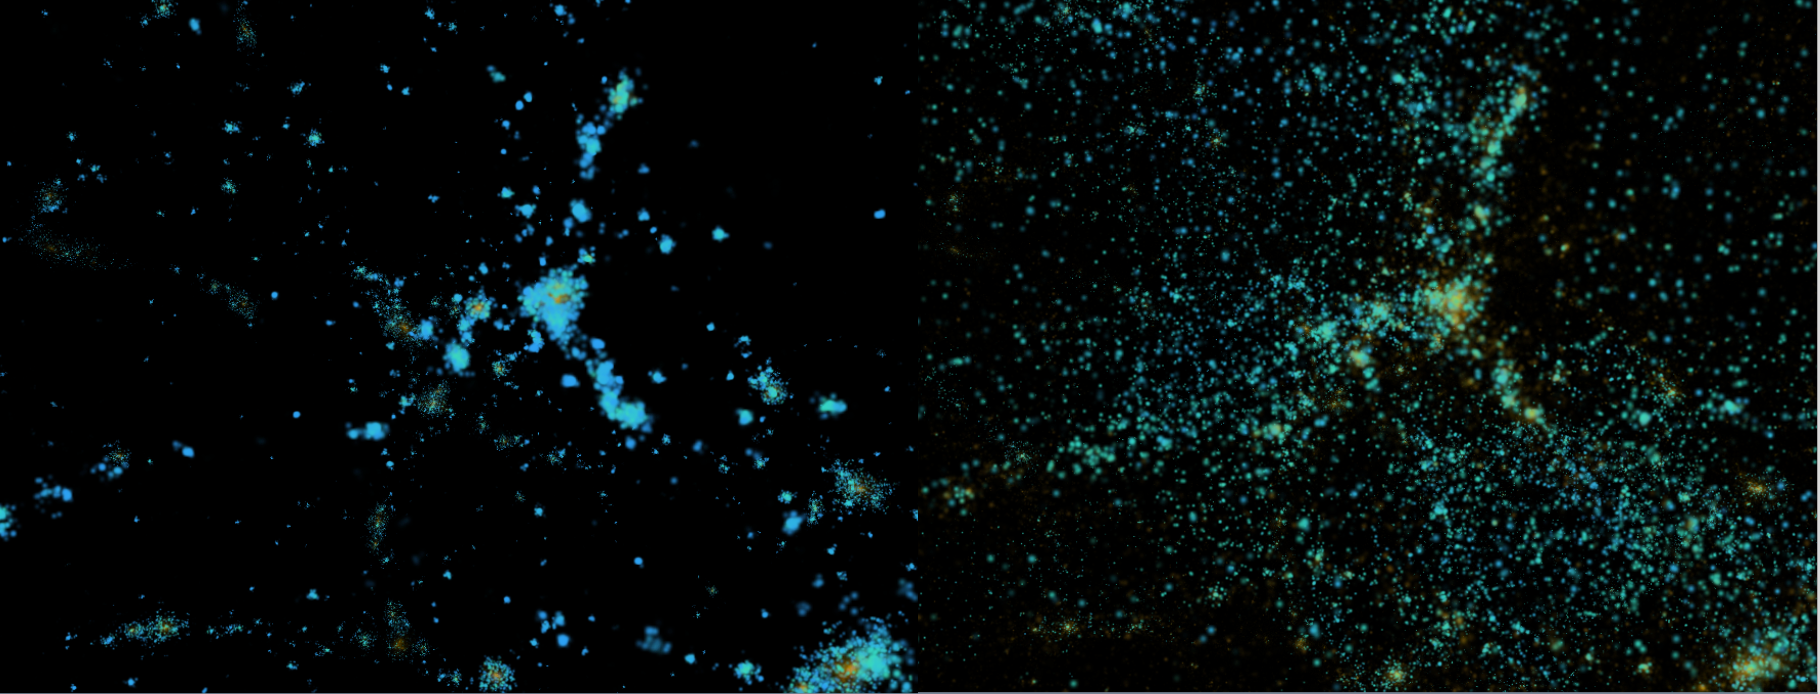
\includegraphics[width=\textwidth]{images/darkmatter/variance_comparison.png}
		\caption{Comparison of different color mappings on particles. Right) Mapping the velocity of the particle. Left) Mapping the variance with the local velocity field. Blue indicates smaller values while green/yellow indicates larger ones.}
		\label{fig:variance_comparison}
	\end{figure}
	
Producing such a view, given the number of particles in each timestep ($\sim 1$ billion), introduces several challenges. First, the user must be able to explore at interactive speeds in order to gain an intuitive understanding of the particle behavior. Second, the merger trees selected by the user may be quite spatially distant from one another, so the entire spatial extent of the domain must be rendered in order to accommodate such requests. Rendering the entire domain also gives crucial global context for areas of interest. To meet these challenges, we incorporate a parallelized particle renderer using a remote server. The rendering server is designed to run on a large visualization cluster and handle data sizes that would be infeasible to render on a single desktop.

\begin{figure}[t]
\begin{center}
$\begin{array}{c}
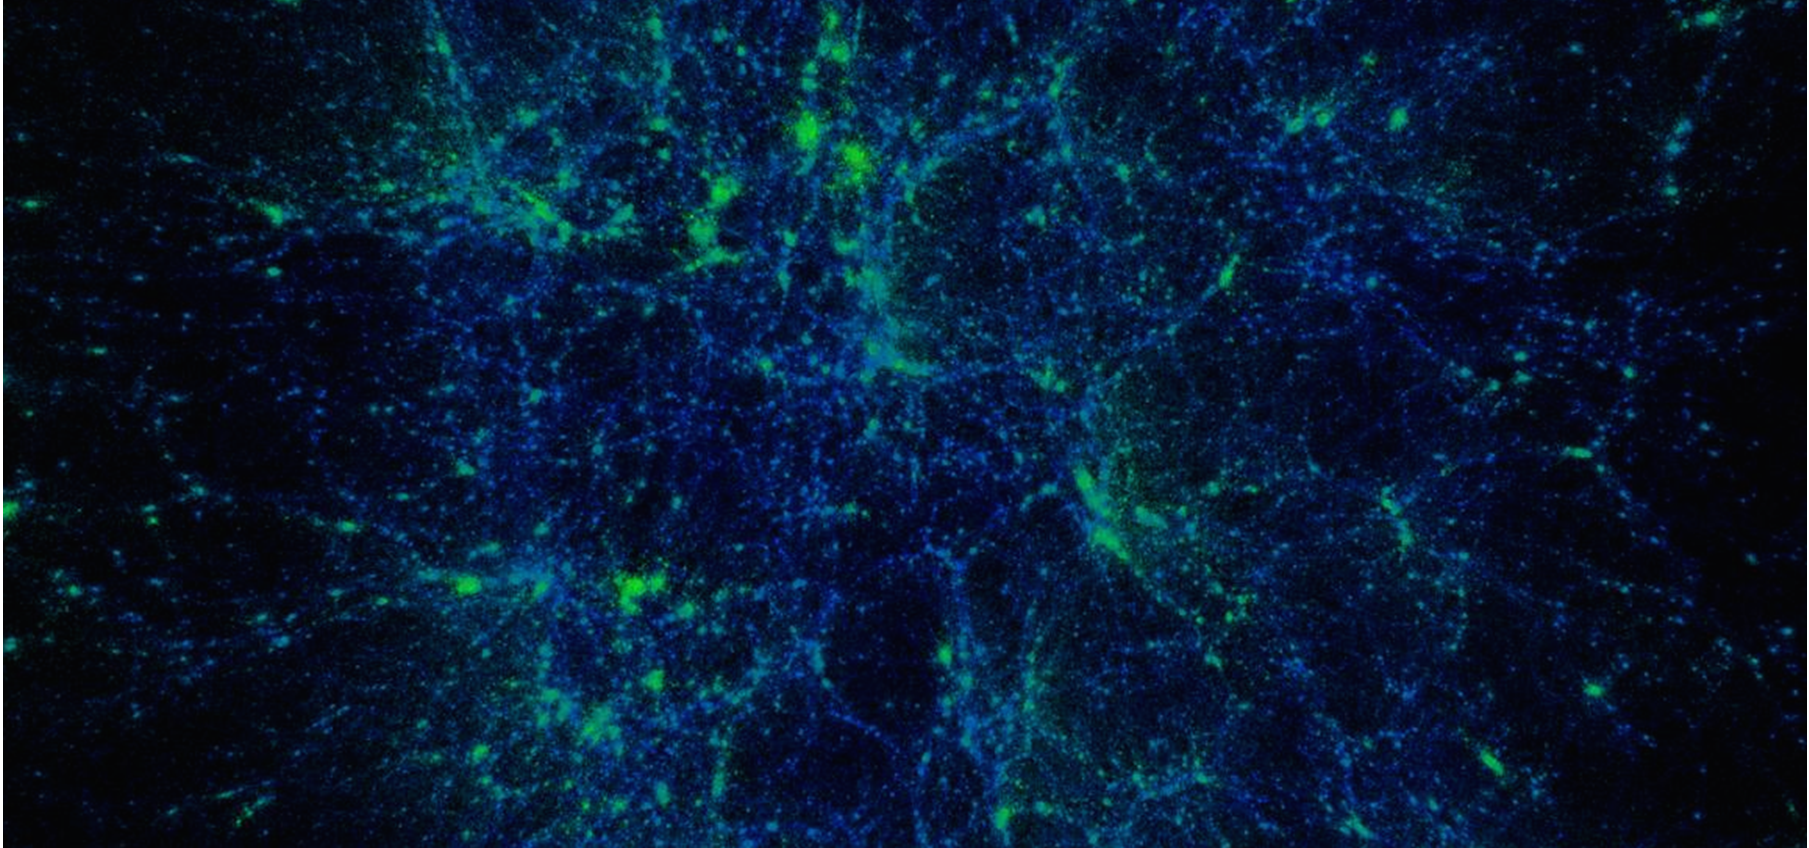
\includegraphics[width=0.95\linewidth]{images/darkmatter/rendering_comparison_b.png}
\vspace{-.05in}
\\
\mbox{\small{(a)}}
\\
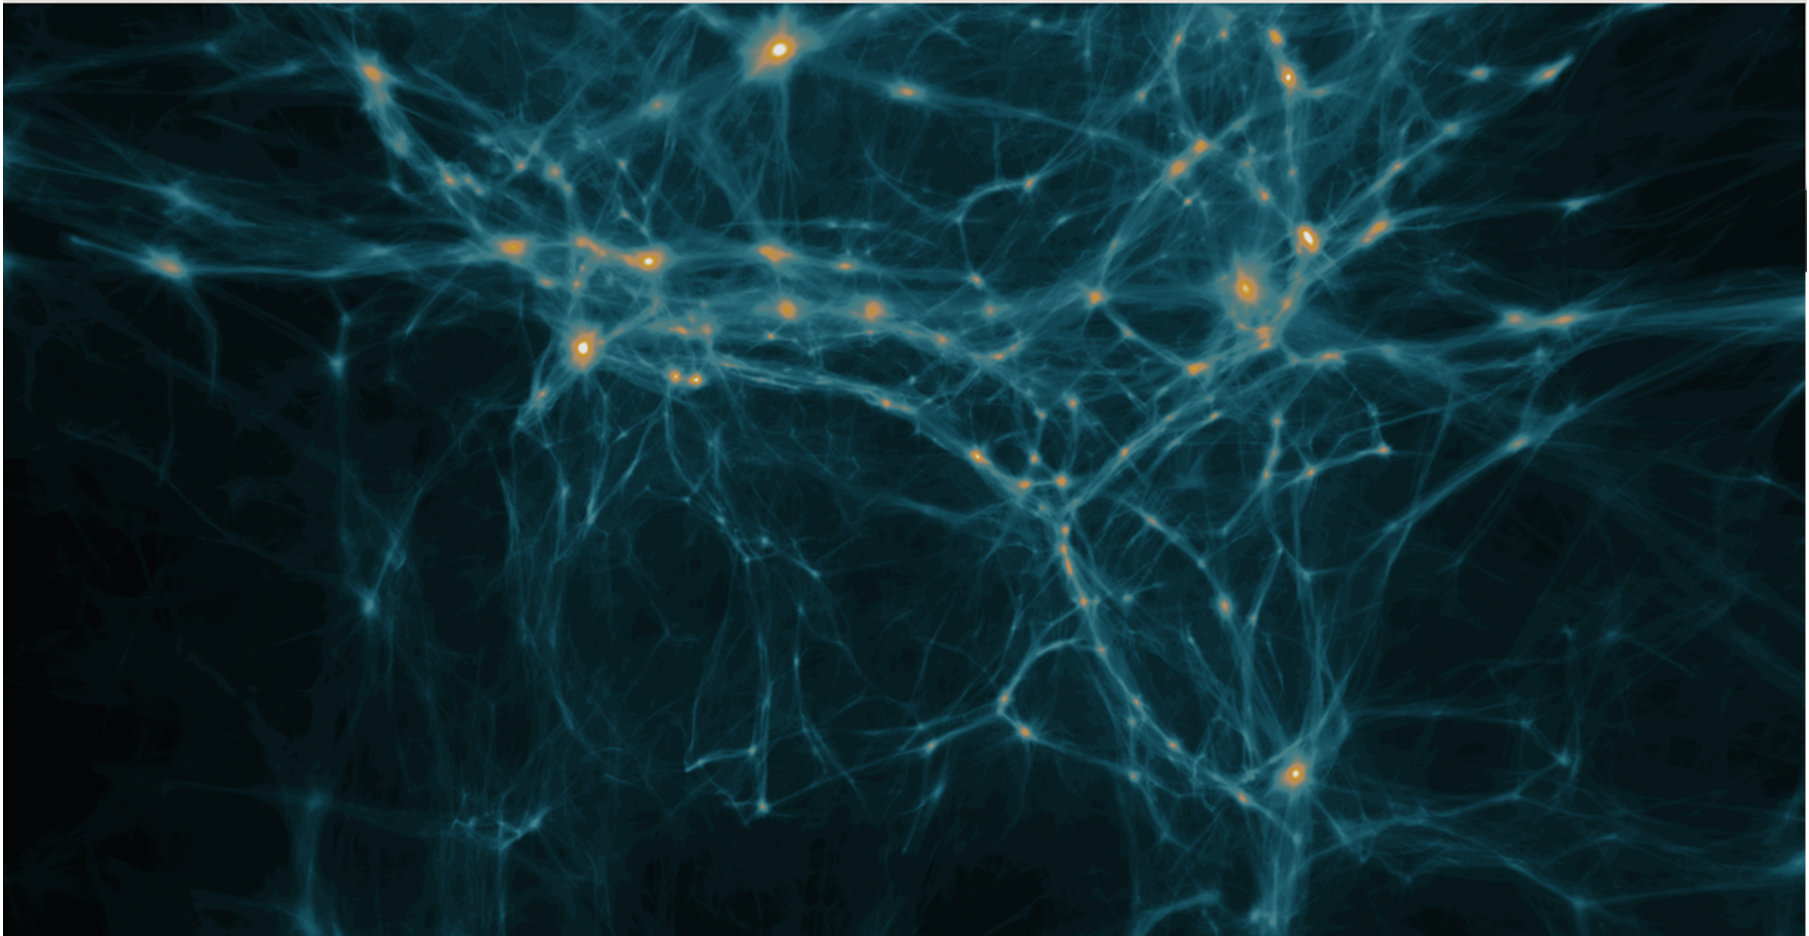
\includegraphics[width=0.95\linewidth]{images/darkmatter/rendering_comparison_a.png}
\vspace{-.05in}
\\
\mbox{\small{(b)}}
\end{array}$
\end{center}
\vspace{-.2in}
\caption{The default particle-based rendering, (a), in comparison with the alternate rendering technique, (b). The default particle view directly conveys data from the simulation, illuminating simulation and analysis code behavior. The alternate technique offers stronger depth cues as well as further insight into the structure of voids and filaments present in the universe.}
\label{fig:comparison_figure}
\end{figure}

In addition to the point-based renderer described above, we also provide an alternate way of visually representing the simulation data. While the point-based approach is useful for visualizing the individual particle locations and distributions when exploring halo substructure, it does not easily portray the filament-like structures that are present in a more macroscopic overview of the data. To address this, we implement another rendering method, which uses a tetrahedral mesh ~\cite{Kaehler:2012}, and allow users to switch between rendering techniques as necessary (Figure~\ref{fig:comparison_figure}).

The main advantage of this technique is that the filament-like structures between larger clusters of matter become obvious to the viewer. One major inaccuracy with N-body simulations comes from the assumption that particles represent a spherical kernel of mass distribution, leading to an exaggeration of gravitational attraction. This may generate extra clumping of particles which compounds on itself as the simulation progresses. The tetrahedral mesh rendering helps to alleviate these inaccuracies through a continuous density approximation of 3D scattered points~\cite{bachthaler2008continuous} and is especially useful in the filament regions. However, this technique is secondary in usefulness to the particle representation, which is directly representative of the data in the simulation and conveys how particles are grouped into halos. Therefore, we use particle splatting as the default method and offer the tetrahedral mesh method as an alternative when desired.

\subsubsection{Quantitative View}
In order to provide quantitative analysis as a complement to the qualitative features of the other views, we incorporate a plot viewer, which utilizes the QCustomPlot library \cite{QCustomPlot}. We employ this view for several specific applications, each extending the usefulness of the two other views with additional quantitative information.

\begin{figure}[t]
        \begin{subfigure}{0.5\textwidth}
        \centering
         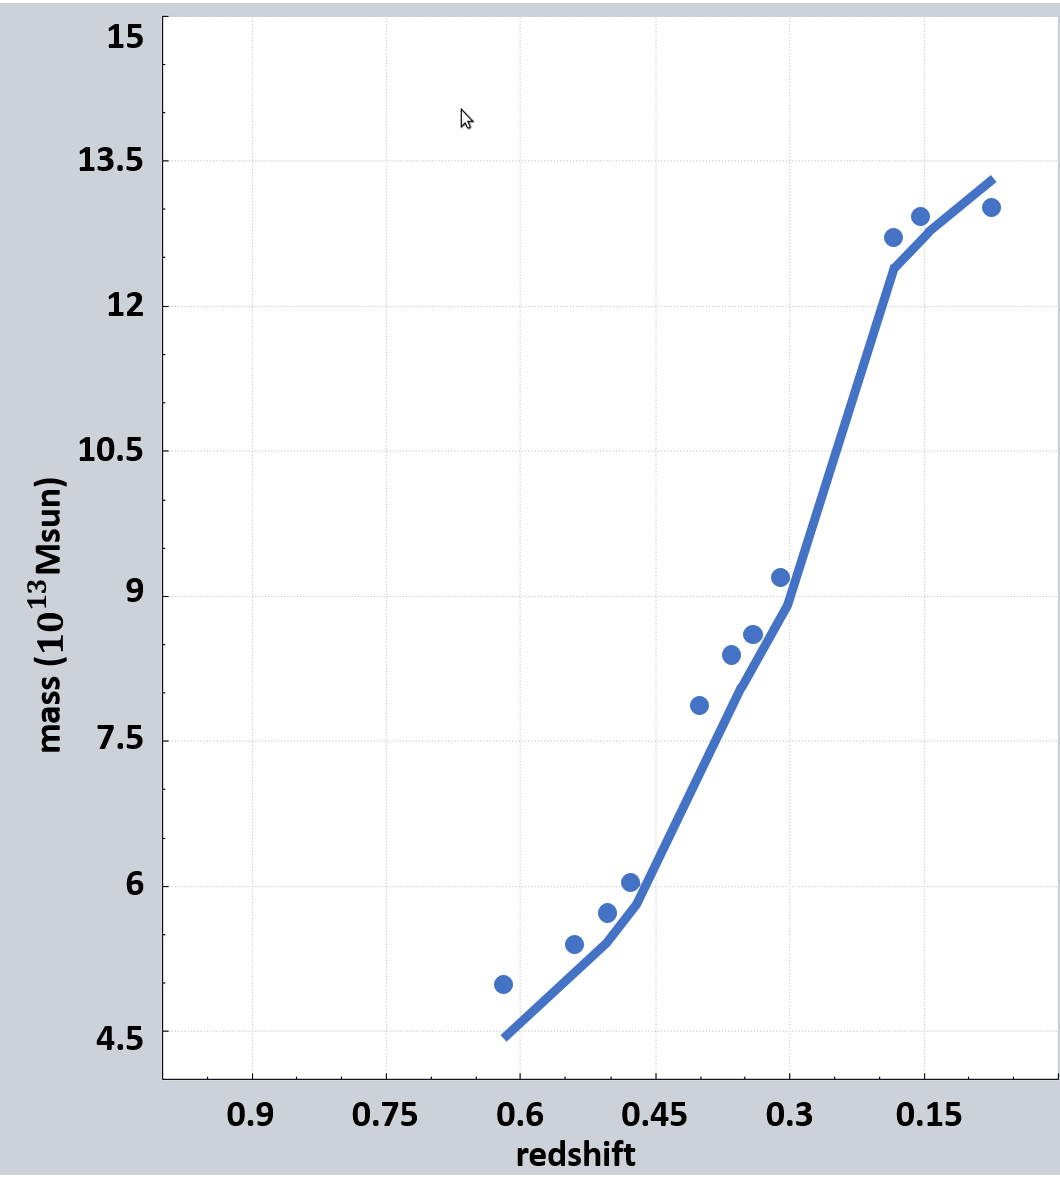
\includegraphics[width=\textwidth]{images/darkmatter/new_plotview_left.png}
                \caption{}
                \label{fig:MPs}
        \end{subfigure}%
        \begin{subfigure}{0.5\textwidth}
        \centering                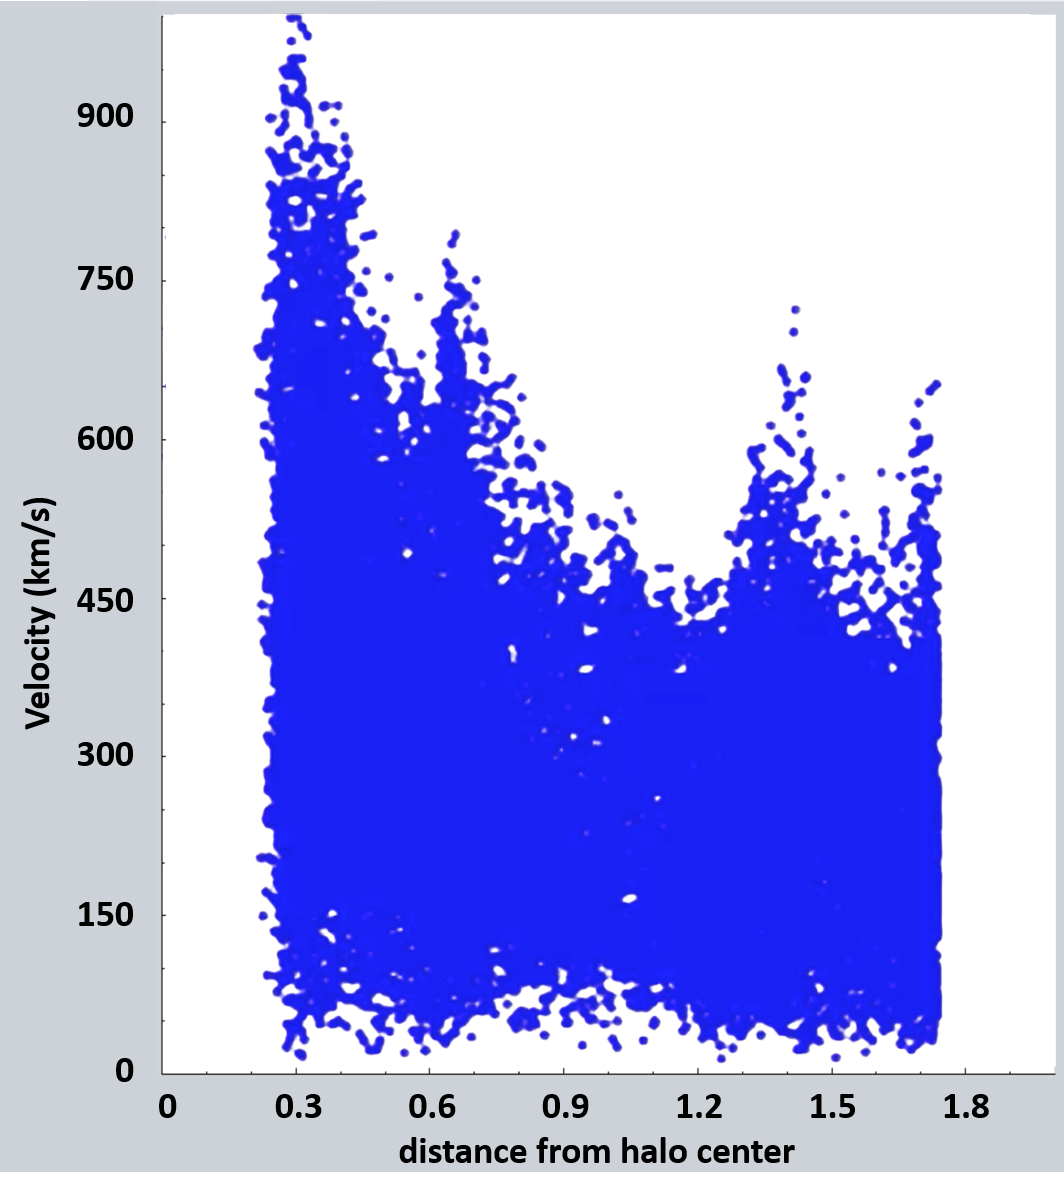
\includegraphics[width=\textwidth]{images/darkmatter/fixed_plotview_right.png}
        \caption{}
        \label{fig:velocity}
    \end{subfigure}
        \caption{The plot view can provides quantitative feedback based on the user's selection in one of the other view spaces. This can reflect selection of a tree in the merger tree view (a), or of a halo in 3D space (b). The left side contains a plot of the missed progenitor history for a selected merger tree. The dots represent anomalous halos; the solid line reflects the sum of the corresponding progenitors. On the right, we plot velocity magnitude vs. distance from halo center, in simulation coordinates, for particles near a selected halo. This local velocity information provides intuition for how the halo is forming; peaks in the plot may indicate substructure.}\label{fig:plots}
\end{figure}

One option given to the user is to view a chronological plot of the anomalous events in a particular halo's history. The system can automatically find instances of events, such as missed progenitors, subject to a user's input threshold. An example of such a plot is shown in Figure~\ref{fig:MPs};  here, a user chooses to locate all nodes for which the sum of the progenitor masses differ from the halo mass by more than $5 \times 10^{12}$ solar masses. Seeing these events chronologically, as well as a quantitative assessment, guides selection for further exploration in the merger tree view.

The user can also choose to see quantitative information about the particles that make up a selected halo. This halo may be selected from the merger tree view or the 3D view. Plotting velocity versus distance from halo center, as the example in Figure~\ref{fig:velocity}, provides additional information about the halo's behavior that is not apparent in the merger tree or 3D views. Such a plot highlights the difference between a stably rotating halo and one in the process of violent mergers. A stable halo should have a relatively continuous velocity distribution, while subhalos interacting with one another will lead to spatially distinct peaks in velocity. This information provides scientists with additional clues as to how structures, such as galaxy clusters, could form in that location.

\subsection{Implementation Details}
The merger trees contain a node for each halo, as well as edges connecting halos with their progenitor and descendant halos. The system reads locally available data, which specifies ID numbers for each halo and its progenitors, and calculates the corresponding tree. This short preprocessing task occurs when the dataset is first loaded.

Our parallel particle renderer performs four steps: data partitioning and loading, local particle splatting, compositing, and sending the resultant image to the client. The data is partitioned into spatially contiguous chunks according to an even subdivision of the particle domain. Although the particle data can be sparse (particularly in later timesteps when dark matter particles have coalesced), it is fairly uniformly distributed for much of the simulation, such that a relatively coarse partitioning with one chunk of particles per rank tends to produce an even load across all ranks. Each chunk is rendered locally on the GPU by splatting its particles to the screen as partially transparent disks~\cite{Gumhold:2003} and blending accordingly. The data chunks are organized into a spatial subdivision tree for easy sorting in view order, and compositing is handled by the 2-3 Swap parallel compositing algorithm~\cite{23swap}. After compositing, the final image is compressed on the head node before being sent over the network to the visualization client. Additional communication between the client and server transmits interactive settings, such as particle selections or color mapping, whenever their values change.

The alternative rendering approach works by treating individual particle locations as vertices of a tetrahedral mesh that is computed in the first timestep of the data. This can be easily determined since the particles are evenly distributed on a near regular grid fashion at the initial condition of the simulation. As the simulation progresses, the tetrahedral mesh becomes deformed as particles move throughout the domain by their gravitational pull and coalesce into halos and larger clusters. These tetrahedra are projected into screen space and are accumulated per pixel to generate an estimate of density in that region. A comparison between this alternate technique and the original point-based method can be seen in Figure~\ref{fig:comparison_figure}.


\section{User Feedback and Results}

We assess our system using data from the Planck simulation run of the HACC framework. This dataset contains 100 timesteps with 1 billion particles ($\sim30$ GB) per timestep. While larger datasets exist, this particular simulation uses a particularly fine mass resolution in order to explore dark matter halo activity in detail. The time ranges from a redshift of $z = 10$ to $z = 0$, which roughly corresponds to 500 million years since the Big Bang, to the present day, about 14 billion years since the Big Bang. The spatial range of the simulation is a cube with sides that are 256 Mpc ($\sim 800$ million light years) in length. This wide temporal and spatial window is important for an accurate simulation, especially because the nature of dark matter and structure formation are largely unknown; scientists cannot safely make assumptions concerning their behavior without simulation data. The merger tree data consists of about 400,000 trees, each representing the evolution of a different halo.

We have consulted closely with several domain scientists, who work with HACC at Argonne National Laboratory, to assess the usefulness of our tool. In general, cosmology researchers are interested in highlighting a specific halo, retrieving relevant information such as its mass, position, or velocity, and tracking descendants and progenitors. The scientists have emphasized that in order to unearth the cause of anomalous merger tree events, it is sometimes necessary to look at how individual halo nodes interact with one another over several consecutive time steps. Thus, our capability for seeing how the halos physically join and split is very useful. When a feature-tracking algorithm returns unpredicted values, numerical analysis alone may not reveal the underlying cause and whether it is a physically feasible event or a feature of the code that needs to be refined. This is especially troublesome because the definitions of mergers, halos, subhalos, and other extracted features may be quite ill-defined. Observing case studies of anomalous events, and seeing the integrated merger tree, quantitative, and 3D views, helps scientists develop and test a hypothesis as to why the simulation data seem to be behaving contrary to physical laws, or to develop an intuition beyond a single numerical model. In addition, our integrated comparison features are useful for data that do not seem to be anomalous. Comparing merger trees for a single halo generated with two different codes, for example, helps qualitatively verify that the outcomes are correct. 

\subsection{Case Studies}

A rigorous definition of a dark matter halo, and the best algorithmic solutions for finding halos and identifying their merger trees, are open-ended areas of active research~\cite{Knebe:2011}. The choice of halo finding algorithm may give inconsistent results or misidentify the behavior of dark matter. To investigate this issue, domain scientists are interested in exploring anomalous nodes in merger trees. These events provide information for further refinement and perfection of their analysis codes. In turn, this visual diagnostic and refinement process will improve the analysis available for large observational surveys such as LSST~\cite{LSST}.

\subsubsection{Heavy Birth Events}

One feature of merger trees that is unreflective of physical laws in reality is the sudden appearance of halos that are well above the simulation's mass resolution. Such an event is unphysical because the particles begin as discrete objects and halo mass must increase continuously over time. This may be caused when a large halo splits into two separate components, such that one of the resulting pieces is identified as having a progenitor and one is not. These scenarios are easy to locate analytically, but it is more challenging to characterize the cause for all of these ``heavy birth'' events. Our linked views provide a way to qualitatively assess such events, verify hypotheses for the inconsistent results, and iteratively refine merger tree code to incorporate this information. The user may see the indication of a heavy birth event in the plot view, select the corresponding node in the merger tree view (Figure~\ref{fig:heavy_birth1}), then refer to the 3D view (Figure~\ref{fig:heavy_birth2}) for information as to why the halo merger code detected an anomalous event. The left side of Figure~\ref{fig:heavy_birth2} shows a ``heavy birth'' halo, and the right side shows this halo in the next timestep, where the halo finder identifies three distinct groups as being in the same halo.

	\begin{figure}[t]
		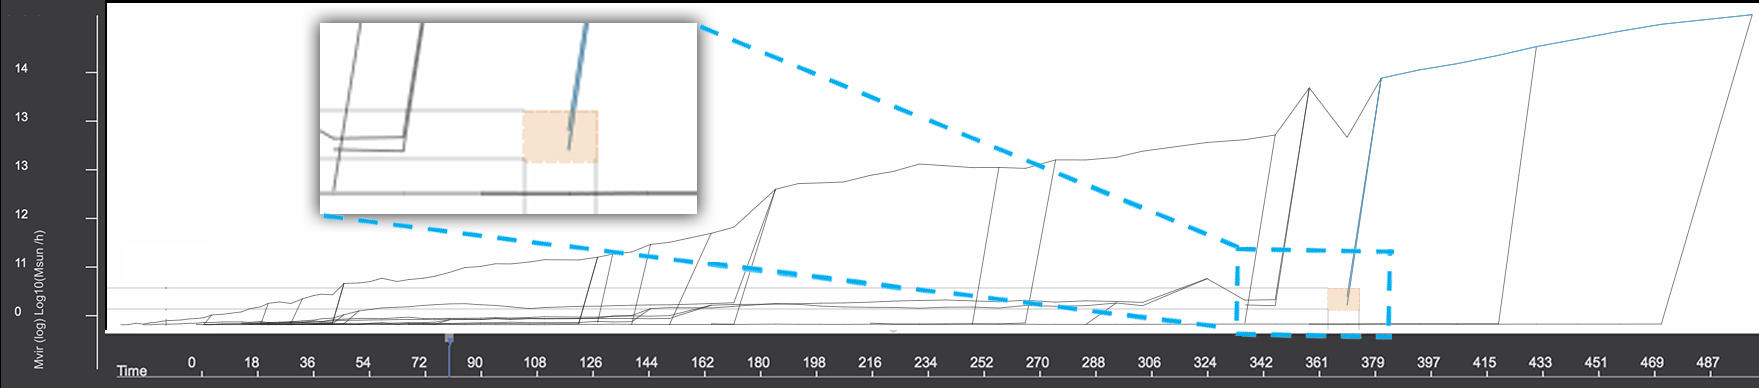
\includegraphics[width=\textwidth]{images/darkmatter/heavy_birth.png}
		\caption{In the merger tree view, the user selects a node with no progenitors that is much more massive than the simulation resolution. This selection triggers highlighting of the relevant particles in the 3D view, seen in this figured in the zoomed-in box.}
		\label{fig:heavy_birth1}
	\end{figure}

	\begin{figure}[t]
		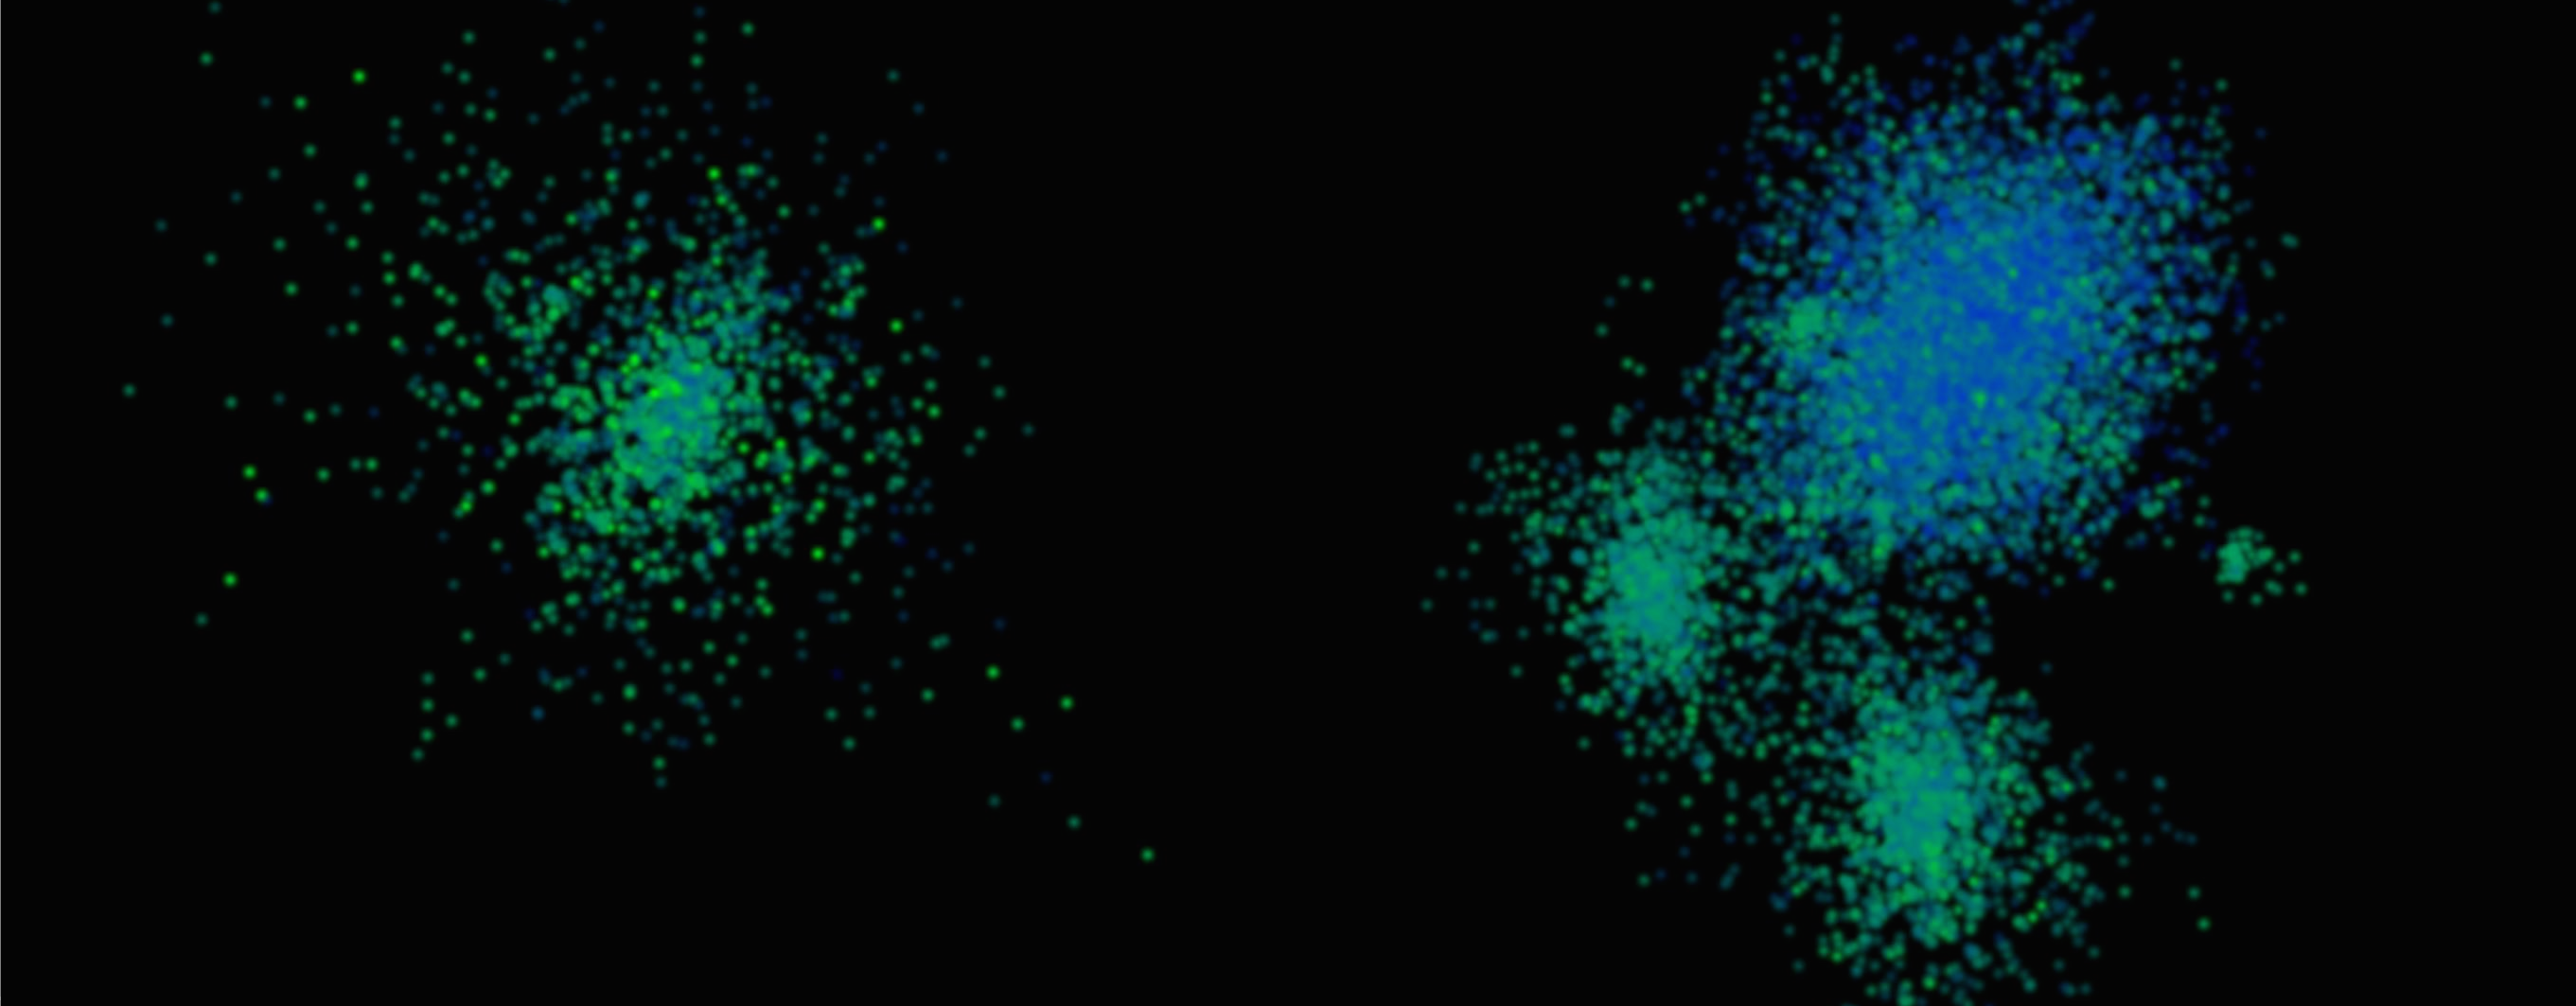
\includegraphics[width=\textwidth]{images/darkmatter/hb_particles.png}
		\caption{Particle data for the selected heavy birth in Figure~\ref{fig:heavy_birth1}. The left image shows the selected halo while the right image shows the same halo a few timesteps later. Note the two satellite halos to the bottom left of the host halo; the halo detection algorithm determines that the halo subsequently grows to include several smaller structures.}
		\label{fig:heavy_birth2}
	\end{figure}

\subsubsection{Missed Progenitors}

The merger tree code may also incorrectly identify a halo and group of progenitors in such a way that the sum of the progenitors' masses differs from the resulting halo's mass by an amount much greater than the simulation's mass resolution. In most of these cases, the total mass of progenitors is less than the halo mass, indicating that one or more halos has been missed by the detection code. 

In the example shown earlier (Figure~\ref{fig:MPs}), the mass of all known progenitors (drawn using a solid line) is noticeably lower than the mass of the resulting halo (drawn as dots) in many timesteps. Moreover, we can see that the mass of the progenitors tends to periodically catch up to the mass of the resulting halo (at $z = 0.45, 0.3, 0.15$ in this case). This pattern could indicate that this merger tree experiences many interactions with other halos. For example, a halo might split apart because of a gravitational interaction, and one resulting piece may join another tree, an event that is difficult to simply characterize using a halo-matching algorithm. In addition, we find that the last timestep results in a halo mass that is less than the sum of its progenitors. Unlike the previous timesteps, the detection code seems to have either identified too many progenitors, or misidentified some heavy halos as progenitors.

%	\begin{figure}[t]
%	\centering
%		\includegraphics[width=3cm]{mp_432.png}
%		\caption{The particles corresponding to the halo represented in Figure~\ref{fig:MPs}. Complex substructure hints at the reason for inconsistent behavior of the halo finding algorithm.}
%		\label{fig:MP_part}
%	\end{figure}

%Figure~\ref{fig:MP_part} shows the corresponding particle data for the halo in question. 
%The high density of particles in this halo coupled with its complex structure could reveal the cause of the discrepancy; perhaps a subhalo is inconsistently being labeled by the code as contained or not contained within the host halo. 

Viewing the corresponding particle data for the halo in question could reveal the cause of the discrepancies; perhaps it contains a subhalo that is inconsistently being labeled by teh code as contained or not contained within the host halo. As with the heavy births, identifying the occurrences of these missed progenitors and further exploring their properties in all three views is essential in correcting and improving merger tree codes. 

\subsubsection{Tidal Disruptions}

After dark matter halos form, they are still subject to gravitational forces from surrounding halos; this may lead to a halo being tidally ripped apart, its particles dispersing in subsequent timesteps. Missed progenitor events, above, may be related to these disruptions. Though such disruptions are certainly physically possible, they are impossible to represent using the current tree structures in which the number of nodes in a tree only becomes smaller over time. Domain scientists are interested in refining their data extraction techniques to take these events into account. Figure~\ref{fig:disruption} shows an example of a tidal disruption candidate that was identified in a preprocessing step. Because one merger tree is inadequate for capturing this event, a user may select nearby halos in the 3D view and inspect their corresponding merger histories or other quantitative information. Through this iterative process, the user can understand how tidal disruptions are characterized in the merger tree framework. The scientists we consulted with are interested in this analysis capability as a basis for developing a new merger tree model that can incorporate halo disruptions.

	\begin{figure}[t]
		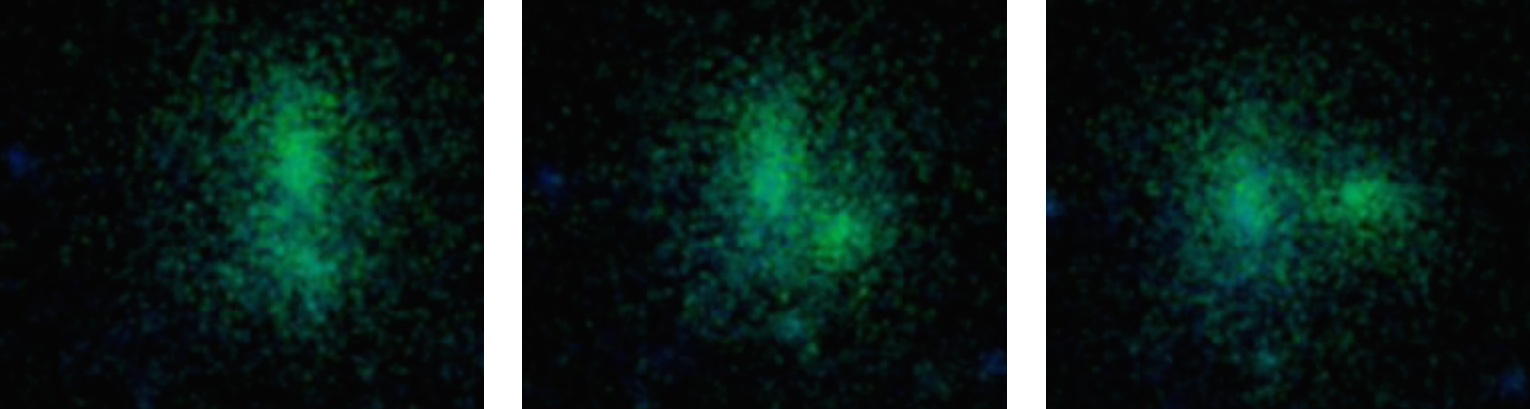
\includegraphics[width=\textwidth]{images/darkmatter/disruption_final.png}
		\caption{Three consecutive snaphsots at late timesteps of a halo that may be experiencing tidal disruption. This is visible in the group of particles that becomes distinct from the host halo over time.}
		\label{fig:disruption}
	\end{figure}

\subsection{Comparative Visualization}

Our system also facilitates visual comparison among data generated using different parameters through a snapshot functionality. Halo finding can be performed with various parameters: for example, the minimum number of particles required to form a halo. In this particular dataset, two sets of merger trees were generated, one with a 10-particle per halo minimum and one with a 100-particle per halo minimum. Figure~\ref{fig:10vs100} compares 10-particle minimum and 100-particle minimum merger trees for the same halo with mass mapped to the vertical axis. The user may choose to save two or more merger trees for comparison in this way, possibly with the corresponding 3D views or quantitative data.

	\begin{figure}[t]
		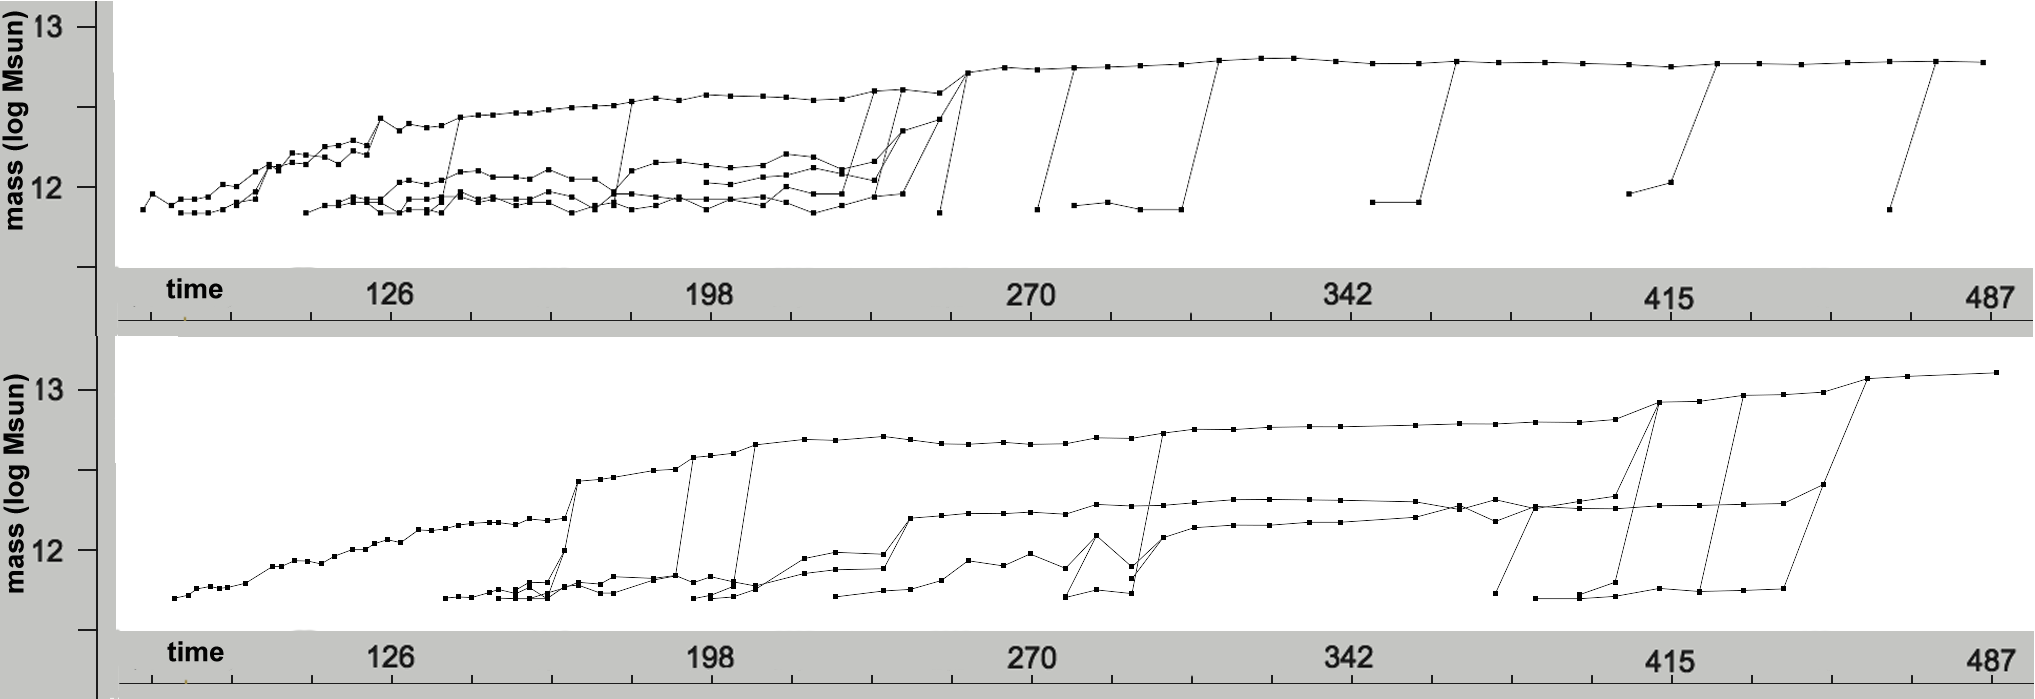
\includegraphics[width=\textwidth]{images/darkmatter/10_v_100_newest.png}
		\caption{Comparison of one merger tree using a 10-particle per halo minimum (top) and a 100-particle per halo minimum (bottom). Because the smaller minimum allows more distinct progenitor halos to be identified early on, the behavior of each tree differs significantly over time.}
		\label{fig:10vs100}
	\end{figure}

From these two images, one can observe how the definition of a halo alters our understanding of the merger tree over time. Though several of the significant merger events are the same in each scheme, the identification of more early progenitor halos using the smaller minimum particle threshold influences the merger tree over time. The higher threshold hides many small halos that may still play a significant role in halo evolution. Observing similarities between these two examples can be used to verify the correctness of the merger tree codes. Moreover, the differences highlighted by this visualization tool can aid scientists in choosing an appropriate balance between the size and resolution of the merger tree data, depending on which halo definition results in merger trees that are more reflective of reality. This comparative visualization makes differences apparent, which may help refine what the correct parameters of a dark matter halo should be, a notion that is still ill-defined~\cite{Knebe:2011}.

	\begin{figure}[t]
		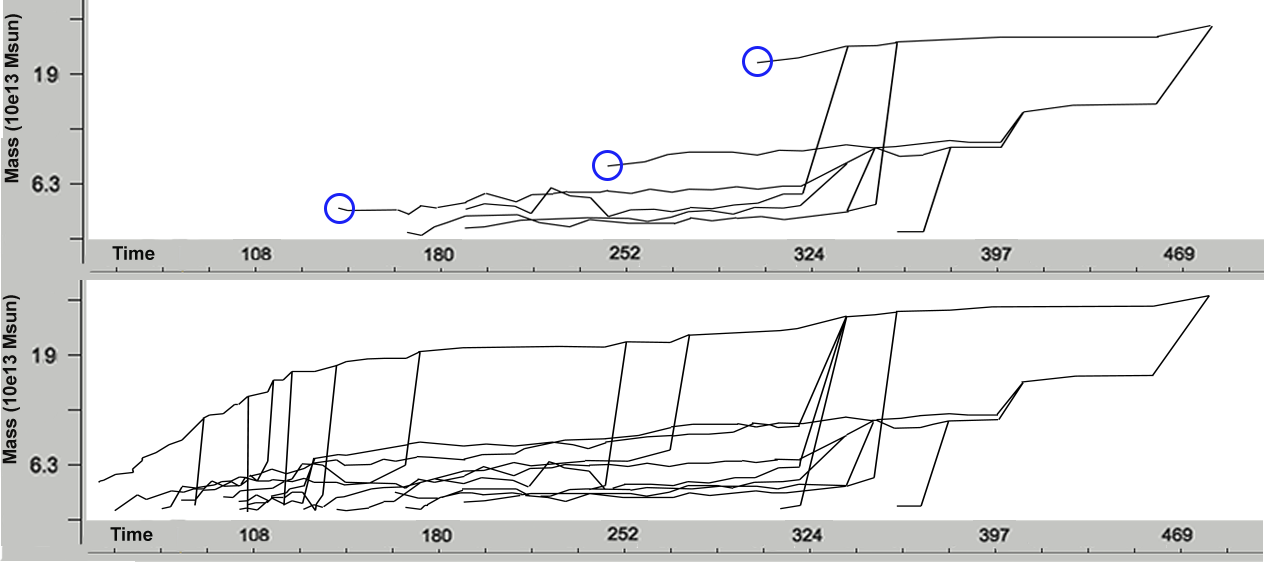
\includegraphics[width=\textwidth]{images/darkmatter/old_vs_new_tree.png}
		\caption{Comparison of two merger trees before (top) and after (bottom) an update to the merger tree finding algorithm. The presence of heavy birth phenomena, circled above in blue, is significantly reduced in the lower tree as very massive halos are now linked to smaller progenitors.}
		\label{fig:oldvsnew}
	\end{figure}

Figure~\ref{fig:oldvsnew} shows another set of merger trees being compared using our system. The top tree shows the presence of many heavy births events. After an update to the merger tree finding algorithm to more carefully account for possible halo splitting, we see significantly fewer heavy births in the lower tree. These are just a few examples of how our visualization tool can provide direct feedback to scientists modifying simulation parameters and algorithms.

\subsection{Performance Results}
The reduced scales of the halo and merger tree data make them easily manageable on a local desktop computer. Furthermore, given the fact the visual clutter will overwhelm users when viewing too many trees at once, only smaller subsets of this data type will be loaded at any given time. As a result, the merger tree and quantitative views are fully interactive with little to no noticeable lag. The particle data is much more massive and requires a distributed framework to render interactively.

The performance and scalability of our renderer was tested on the Cooley visualization cluster at Argonne National Laboratory. Cooley has 126 nodes, connected via a FDR Infiniband interconnect. Each node has 12 CPU cores at 2.4 GHz, 384 GB of RAM, and a NVIDIA Tesla K80. GPU memory is the theoretical limit for the number of particles we can allocate each GPU, but in practice, one would lose interactivity long before running out of memory. When running, we allocate two ranks per node, and assign one rank to each GPU.

\begin{figure}[t]
	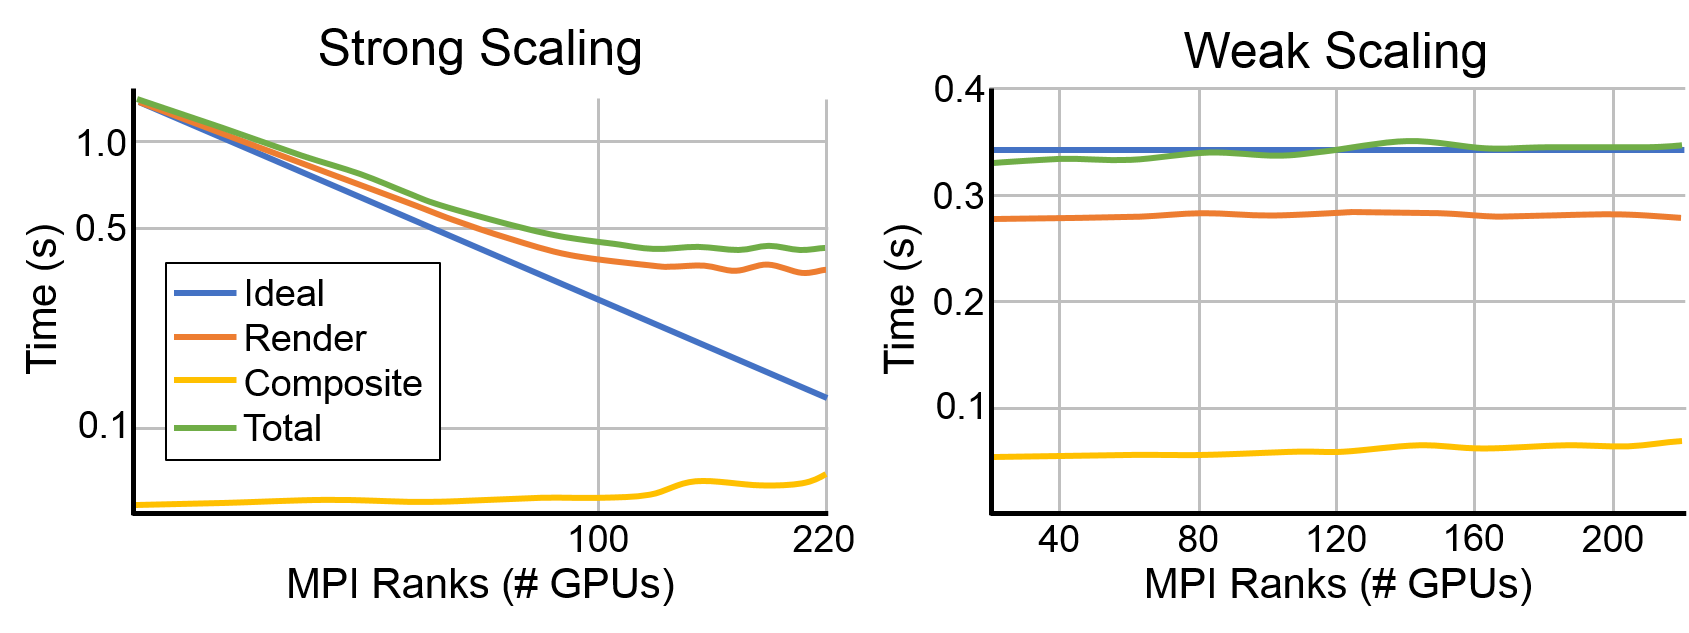
\includegraphics[width=8.5cm]{images/darkmatter/test_scaling2.png}
	\caption{The log/log plot of strong scaling results for our system (left) shows a decrease in performance at large numbers of nodes, indicating an overhead cost of the renderer. Weak scaling (right) shows nearly ideal total rendering time across all machine sizes.}
	\label{fig:scaling}
\end{figure}

We conducted strong and weak scaling studies to assess our system (figure~\ref{fig:scaling}). The ideal time is defined as $t_0 / N$ for strong scaling, and $avg(t_0, t_N)$ for weak scaling, where $t_i$ is the total time for the machine size $i$, and $N$ is the maximum machine size used in our study (220 GPUs). Each measurement is the average of 42 views evenly distributed around the outside of the data volume in order to make the time measurements view-independent. The full data was used for every machine size in the strong scaling study. The number of particles per node for the weak scaling study, 5368619, was kept constant by partitioning the data as normal, then selecting a random subset of the particles from the partition assigned to each node.

Our strong scaling results show good scaling for this dataset up until 80 nodes, after which our times diverge from ideal scaling. We believe this is due to a constant overhead cost in our renderer, and that there is room for optimizations to reduce this overhead. The weak scaling results, where the total rendering time is close to the ideal scaling time across all machine sizes, reflect the scalability of our system.

\section{Discussion}
We designed our tool so that it has the flexibility to visualize cosmological data from sources other than HACC. Since data from many other cosmology simulations are similarly split into the particle, halo, and merger tree representations, our visualization tool can not only be used to compare results between different runs of a simulation, but also between different types of simulations. This comparison can be useful when comparing different computational models of universe formation, such as comparing an N-body gravitational simulation with one that includes hydrodynamic effects.

Our ability to interactively explore the large datasets produced by simulations in the HACC framework demonstrates our tool's scalability. The remote particle renderer allows for the visualization of even larger datasets: additional particles can be included with very little increase in overhead by incorporating additional computing nodes. The highly parallel nature of distributed particle rendering ensures that communication costs between nodes can be kept small.

Future simulations, with finer mass resolution and more particles, will produce too many merger trees to be handled efficiently at a local level. Therefore, we plan to implement all three visualization views in a remote and parallelized setting. In this scheme, all data produced by the simulation can remain in place while analyzed remotely from a desktop computer. This will reduce the I/O costs associated with data transfer between different locations. 
Due to the highly interconnected halo, progenitor, and descendant data, implementing the merger tree view in a distributed manner can result in large communication costs between computing nodes. In order to maintain interactive speeds, some form of node-level data redundancy may need to be implemented for this view.

Interactive analysis of cosmological simulation data is vitally important to preparing for upcoming large-scale astronomical surveys~\cite{skysurvey}. It is important to hone an accurate model of structure formation in the universe, which astronomers believe is dictated by the evolution of dark matter halos. Because these halos cannot be directly observed, a solid theoretical understanding, guided by simulations, is necessary to link theory with observational data. If correct, these simulations should produce results, such as the mass and brightness distributions of galaxies, that match those observed in surveys. Any differences between the two may point to a further refinement of simulation algorithms.

Flow visualization is another broad area that can benefit from such a visualization tool. The large particle-based data in Lagrangian flow representations can be visualized using our parallel particle renderer. Any accompanying Eulerian features and regions of interest that are identified and tracked throughout the simulation can also be displayed using our merger tree visualization. Moreover, linking these views can enhance the exploration of particle and feature correspondence and lead to finer understanding of underlying processes.

\section{Conclusion and Future Work}

We have created a system for interactive analysis of large cosmological simulation data. By linking views of multiple simulation data types, we offer an opportunity to gain new intuition for simulation code behavior and for features of interest in the universe.

Due to the very large, and increasing, scales of simulation and observational data, future work must focus on improved capability for interacting with large data sets. In particular, we hope to work with a larger version of the data set addressed in this paper, and include capability for smooth animation over several time steps. We also aim to provide improved capacity for viewing quantitative information from throughout a halo's history, which is costlier to look up than data from the present time step.

The application of visual diagnostics to cosmological datasets has vast potential for future work. In addition to refining merger tree models for the evolution of dark matter halos, scientists also seek to characterize specific properties of halos, such as their alignments and centers of mass \cite{Behroozi:2013}. The calculation of minimum potential needed to find halo centers is expensive, and the result is likely to change drastically depending on the properties of the halo-finding algorithm. Visual analysis, with a complementary 3D view and quantitative information, would help troubleshoot the results of center-finding codes. There is also great interest in exploring related topics such as multi-streaming and structure formation events \cite{Popov:2011}, and using semi-analytic models to superimpose galaxy information onto dark matter simulation data, which may then be compared directly to observations. With help from visual diagnostics, the trend towards accuracy in cosmological simulation analysis will enhance scientists' abilities to learn from the largest, most ambitious observational sky surveys.